\documentclass{article}

% Set page size and margins
% Replace `letterpaper' with `a4paper' for UK/EU standard size
\usepackage[letterpaper,top=2cm,bottom=2cm,left=3cm,right=3cm,marginparwidth=1.75cm]{geometry}
\usepackage[spanish]{babel}
\usepackage{url}
\usepackage{hyperref}
\usepackage{csquotes}
\usepackage{amsmath}
\usepackage{amssymb}
\usepackage{graphicx}
\usepackage{listings}
\usepackage{xcolor}
\usepackage{setspace}
\usepackage{float}

\graphicspath{ {assets/} }

%Code colors:
\definecolor{codegreen}{rgb}{0,0.6,0}
\definecolor{codegray}{rgb}{0.5,0.5,0.5}
\definecolor{codepurple}{rgb}{0.58,0,0.82}
\definecolor{backcolour}{rgb}{0.95,0.95,0.92}
\doublespacing

\lstdefinestyle{mystyle}{
    backgroundcolor=\color{backcolour},
    commentstyle=\color{codegreen},
    keywordstyle=\color{magenta},
    numberstyle=\tiny\color{codegray},
    stringstyle=\color{codepurple},
    basicstyle=\ttfamily\footnotesize,
    breakatwhitespace=false,
    breaklines=true,
    captionpos=b,
    keepspaces=true,
    numbers=left,
    numbersep=5pt,
    showspaces=false,
    showstringspaces=false,
    showtabs=false,
    tabsize=2
}

\lstset{style=mystyle}

\NewDocumentCommand{\codeword}{v}{%
    \texttt{\textcolor{black}{#1}}%
}

\begin{document}

    \begin{titlepage}
        \centering
        {
\includegraphics[width=0.5\textwidth]{logo2}\par}
        {\bfseries\LARGE Universidad Católica del Uruguay \par}
        \vspace{0.3cm}
        {\scshape\Large Facultad de Ingeniería \par}
        \vspace{0.3cm}
        {\scshape\Huge Proyecto \\Tarea 1 - Análisis de Sentimientos \par}
        \vspace{1cm}
        {\Large Álgebra Aplicada \par}
        {\Large Profesor: Maglis Mujica \par}
        \vfill
        {\Large Autores: \par}
        {\Large Piero Saucedo (5.342.503-5)\\Juan Martín Riccetto (5.324.939-0)\\Juan Manuel Perez (4.673.899-0) \par}
        \vfill
        {\Large \today \par}
    \end{titlepage}

    \section{Introducción}\label{sec:introduccion}
    En el marco teórico de Álgebra Aplicada, se propone a los estudiantes una tarea centrada en el uso de vectores.

    En esta ocasión, el objetivo principal es, dado un número de 15 frases seleccionadas, armar un modelo
    vectorial en base a palabras “clave”, que se vean repetidas a lo largo de las mismas, además estas palabras
    claves son clasificadas dentro de los grupos “positivas”, “neutrales” y “negativas”, de forma que sea posible
    estudiar distintas características de las frases mencionadas.

    \section{Marco Teórico}\label{sec:marco-teorico}
    Este marco teórico pretende proporcionarle al lector una compresión de los conceptos utilizados durante el
    desarrollo de la tarea, por lo que se abarcarán aquellos pertinentes a la misma.

    \subsection{Vector}\label{subsec:vector}
    Un vector es una entidad matemática que tiene magnitud y dirección.
    Es una herramienta fundamental en matemáticas y física, utilizada para representar cantidades que no solo tienen
    un tamaño (magnitud), sino también una dirección.

    Un vector con un origen fijado queda determinado a partir de dos elementos:
    \begin{itemize}
        \item Una \textbf{semirrecta} partir de dicho origen, es decir, una dirección hacia la que apunta.
        \item Un número no negativo, llamado \textbf{módulo} del vector y que mide su tamaño.
    \end{itemize}

    Alternativamente, se puede fijar un sistema de coordenadas del espacio \textit{n} \textit{n-dimensional};
    entonces un vector queda unívocamente determinado mediante \textit{n} números, llamados coordenadas del vector.

    \section{Objetivos}
    \begin{itemize}
        \item Obtener diferentes frases publicadas en línea con ciertas palabras claves en común.
        \item Extraer una serie de palabras claves que sirvan de indicio para clasificar a las frases
        por una determinada connotación.
        \item Analizar los enunciados recolectados con el fin de obtener distintos datos sobre los mismos en base a las palabras claves que posean.
    \end{itemize}

    \section{Desarrollo}
    \subsection{Frases Elegidas}
    Elegimos una serie de quince frases ficticias para ser procesadas:
    \begin{itemize}
        \item ``Acabo de ver \textit{Inception} otra vez. Cada vez me deja con más preguntas... ¡Es una locura!''
        \item ``Me encantó \textit{Barbie}! No esperaba que fuera tan divertida y profunda al mismo tiempo.''
        \item ``La cinematografía de \textit{Dune} es impresionante, pero siento que la historia se quedó corta. ¿Alguien más piensa lo mismo?''
        \item ``¿Alguien más lloró viendo \textit{Coco}? Esa película siempre me llega al corazón.''
        \item ``No puedo superar lo épico que fue el final de \textit{Avengers: Endgame}. Todavía me da escalofríos.''
        \item ``¡Qué decepción fue \textit{Morbius}! Esperaba mucho más de esta película.''
        \item ``Las películas de terror ya no son lo que eran... Vi \textit{Smile} y fue predecible en casi todo.''
        \item  ``Acabo de ver \textit{El Padrino} por primera vez. Ahora entiendo por qué es un clásico, ¡es una obra maestra!''
        \item ``¡Me encantó \textit{Spider-Man: No Way Home}! La nostalgia me pegó fuerte, ¡qué momentos!''
        \item ``Las películas de \textit{Studio Ghibli} son arte puro. \textit{El Viaje de Chihiro} es mi favorita de todas.''
        \item ``Nunca pensé que \textit{Oppenheimer} sería tan fascinante. La historia te mantiene enganchado desde el principio.''
        \item ``¡Qué sorpresa fue \textit{The Menu}! No esperaba que la película tuviera tantas capas de significado.''
        \item ``Creo que \textit{John Wick} es la mejor saga de acción de esta década. Las coreografías de pelea son impresionantes.''
        \item ``¿Soy yo o \textit{Tenet} fue demasiado complicada de entender? Necesito verla de nuevo para captar todo.''
        \item ``El remake de \textit{La Sirenita} fue hermoso. Me encantó cómo mantuvieron la esencia del original, pero con un toque moderno.''
    \end{itemize}

    \subsection{Palabras Clave}
    \begin{itemize}
        \item \textbf{Positivas:} encanto, fascinante, épico, hermoso, impresionante, divertida, mejor, moderno
        \item \textbf{Neutrales:}  preguntas, esperaba, siento, necesito, pienso, piensa, puro, enganchado, profunda, clásico
        \item \textbf{Negativas:} complicadas, decepción, predecible, corta, locura, lloró, fuerte

    \end{itemize}

    \subsection{Funcionamiento del código}
    \begin{figure}[H]
        \centering
        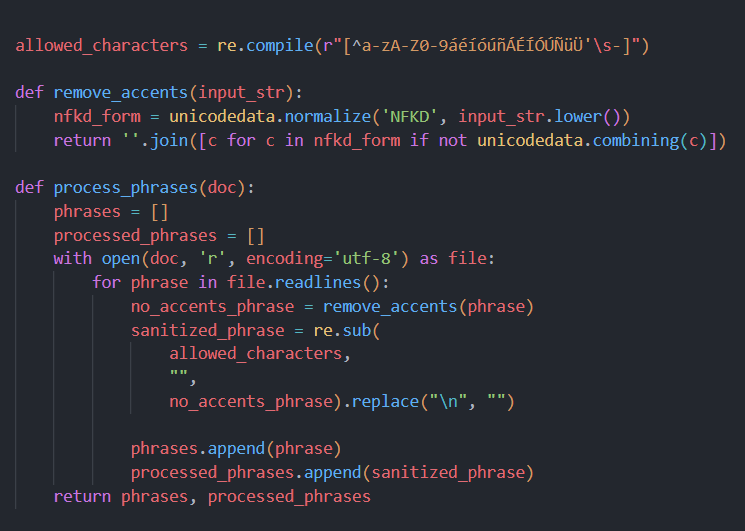
\includegraphics[width=1\linewidth]{assets/Codigo1}
    \end{figure}
    La primera parte del código sanitiza las frases elegidas de forma que sean más fáciles de manejar y analizar.\\

    \begin{figure}[H]
        \centering
        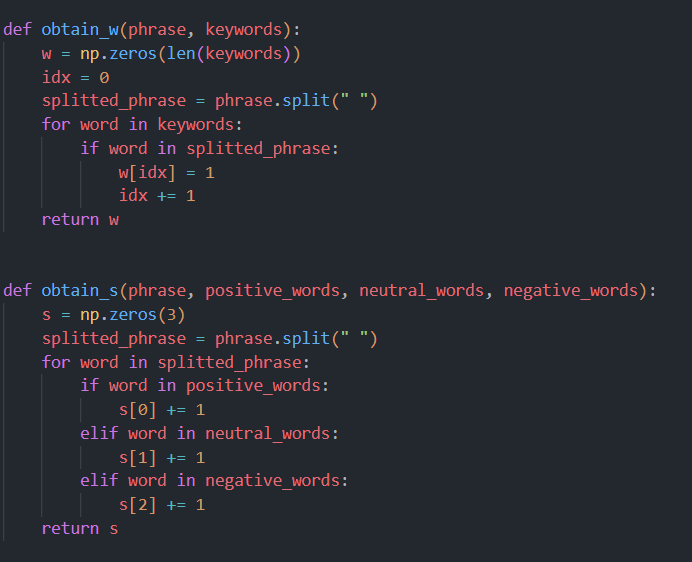
\includegraphics[width=1\linewidth]{assets/Codigo2}
    \end{figure}
    Estas funciones toman las frases sanitizadas y las palabras claves para formar los vectores w y s respectivamente, cuando se encuentra una palabra clave se suma 1 al indice correspondiente.\\

    \begin{figure}[H]
        \centering
        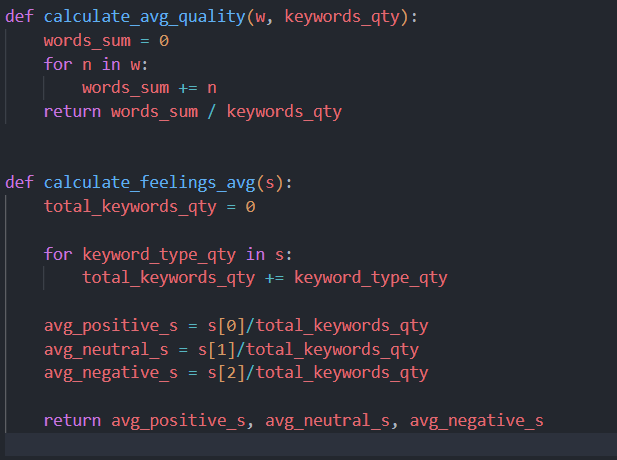
\includegraphics[width=1\linewidth]{assets/Codigo3}
    \end{figure}
    Aquí se ven las funciones para calcular la calidad promedio y el promedio de sentimientos de cada frase, la primera función toma todas las palabras claves encontradas y las divide entre las palabras clave totales.
    La segunda función, separa las palabras clave dentro de las frases en positivas, neutrales y negativas, y divide cada grupo entre las palabras totales encontradas en la frase.\\

    \begin{figure}[H]
        \centering
        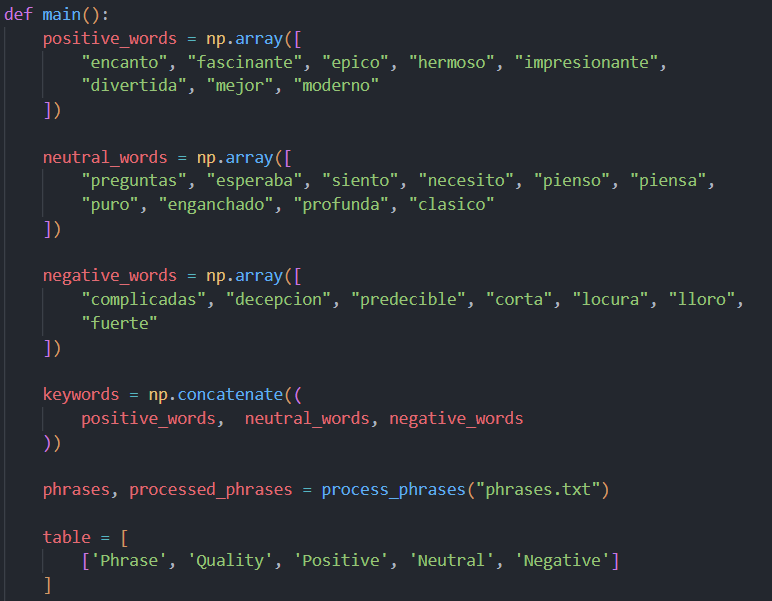
\includegraphics[width=1\linewidth]{assets/Codigo4}
    \end{figure}
    En el main se definen vectores para cada uno de los tipos de palabras clave y se crea otro que contenga la totalidad de las mismas. Además se crea una variable que contenga las frases procesadas, y una tabla en la que se mostrarán sus atributos.\\

    \begin{figure}[H]
        \centering
        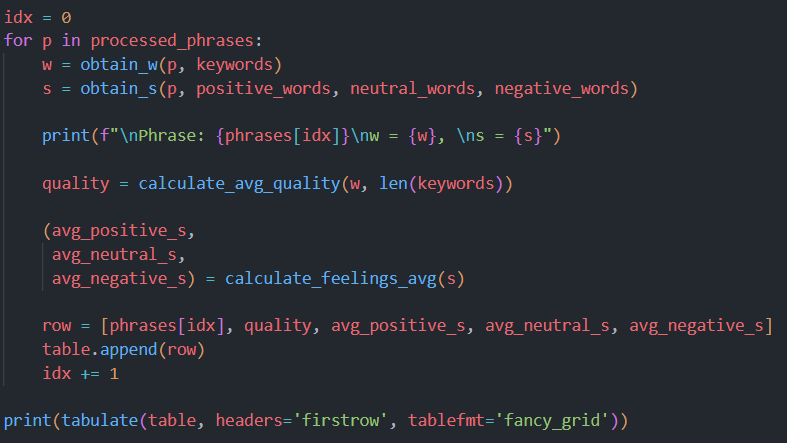
\includegraphics[width=1\linewidth]{assets/Codigo5}
    \end{figure}
    Por último se corren todas las funciones mencionadas previamente y se imprimen los resultados.\\
    
    \subsection{Calidad Promedio y Promedio de Sentimientos}
    \begin{figure}[H]
        \centering
        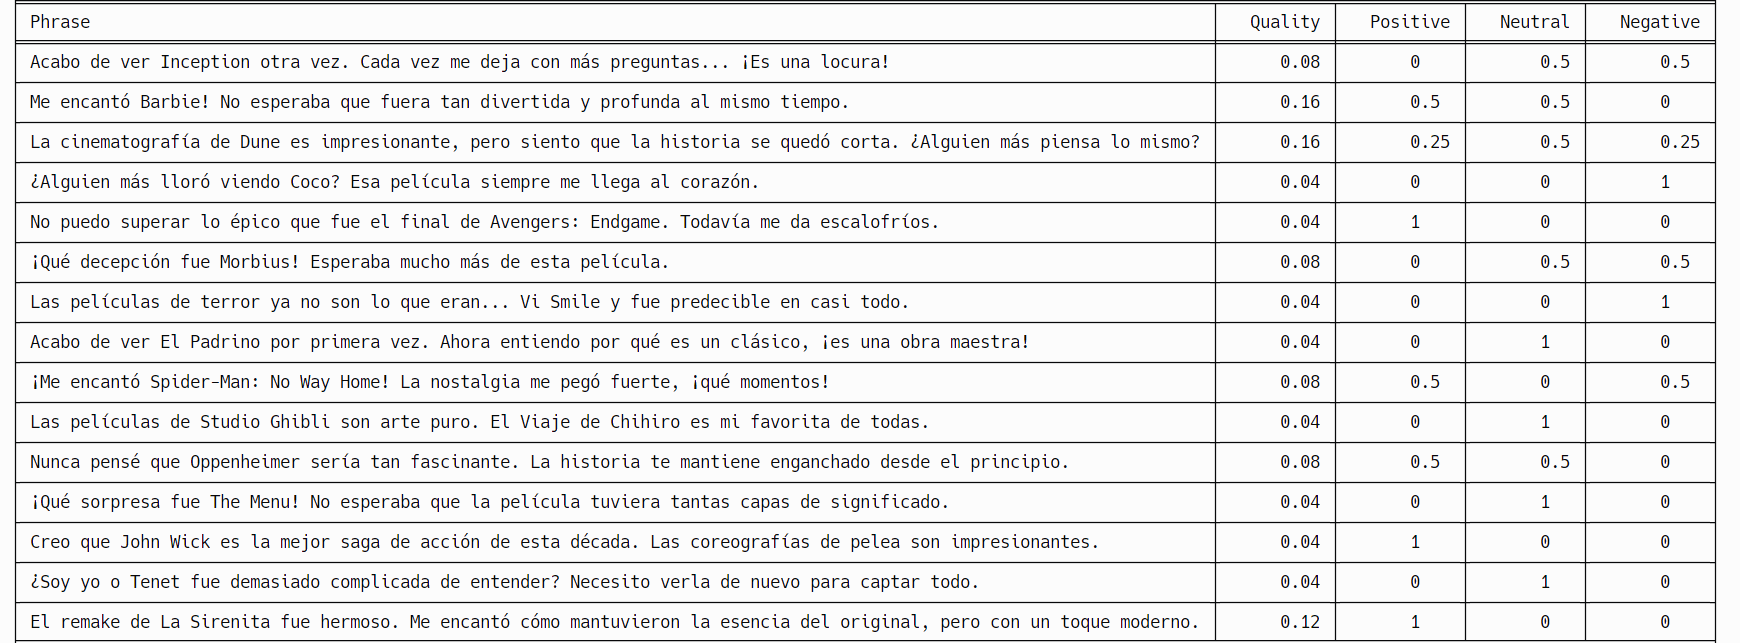
\includegraphics[width=1\linewidth]{assets/results}
    \end{figure}


    \subsection{Frase más positiva}
    Las frases 5, 13 y 15 son las más positivas, todas con un valor de 1.

    \subsection{Frase más negativa}
    Las frases 4 y 7 son las más negativas, ambas con un valor de 1.

    \subsection{Calidad Promedio}
    La calidad promedio puede verse también como el porcentaje de palabras claves contenidas en cada enunciado, por ejemplo la frase 2 tiene una calidad promedio de 0.16, que podría ser visto como 16\%, de la misma manera, si una frase contuviera el conjunto entero de palabras clave, su calidad promedio sería de 1.00 o 100\%.

    \subsection{Promedio de Sentimiento}
    El promedio de sentimiento, se puede resumir en el porcentaje de una frase en un sentimiento específico con respecto al resto, o en otras palabras, se toma el total de palabras claves dentro de una frase, y divide la cantidad de palabras de un sentimiento específico. En el caso de que una frase contenga únicamente palabras positivas, su promedio de sentimiento positivo será 1.00 o 100\%, o en el caso de que haya una cantidad uniforme de palabras para cada sentimiento, los tres receibirán un valor de 0.33 o 33\%.

    \subsection{Impacto de las palabras claves}
    Sin duda son las palabras claves las que moldean los resultados provistos por el algoritmo, con solo cambiar un par de estas, desencadenaría tanto en calidades promedio como promedios de sentimiento completamente distintos para la gran mayoría sino todas las frases selectas.

    \subsection{Optimizaciones}
    En general, podría optimizarse el código reemplazando varios de los loops dentro del mismo, con operaciones vectorizadas de la librería NumPy, esto si nos reducimos solo a la parte del propio algoritmo.

    Si nos vamos a la parte del análisis en sí, hay varias formas de mejorarlo, especialmente mediante el uso de técnicas de aprendizaje automático (\textit{Machine Learning}). Los modelos supervisados como \textbf{Naive Bayes}, \textbf{Support Vector Machines (SVM)} y \textbf{Logistic Regression} pueden entrenarse con conjuntos de datos etiquetados para identificar patrones de sentimiento en las frases, ofreciendo una precisión superior en comparación con las técnicas basadas en reglas.

    Ampliar el conjunto de datos puede ser otra estrategia valiosa. Utilizar un vocabulario más extenso, puede mejorar la capacidad del modelo para interpretar frases. La creación de un conjunto de datos etiquetado manualmente también serviría como una base sólida para entrenar modelos supervisados.

    \section{Conclusiones}
    Concluimos entonces que el análisis de las frases proporcionadas utilizando técnicas de procesamiento del lenguaje natural y la implementación de un modelo de clasificación de sentimientos ha resultado exitoso. Se lograron clasificar las frases de manera efectiva en las categorías de positiva, negativa y neutral, lo que permitió obtener una visión clara de las emociones subyacentes en las expresiones del autor sobre diferentes películas.

    Las frases con una connotación positiva están asociadas principalmente con películas que evocaron fuertes emociones, nostalgia, y sorpresas agradables. Estas frases destacan apreciaciones por la profundidad temática, la calidad cinematográfica y la capacidad de las películas para involucrar emocionalmente al espectador.

    Por otro lado, las frases con una connotación negativa tienden a centrarse en la falta de innovación, predecibilidad o en experiencias que no alcanzaron las expectativas generadas. Esto refleja una sensibilidad del autor hacia la originalidad y la calidad narrativa en las películas que consume.

    Esto evidencia la utilidad de los vectores en este tipo de aplicaciones; es decir, cómo, utilizando conceptos puramente matemáticos (algebraicos, más específicamente), se puede obtener información valiosa que puede ser provechosa para el análisis de datos.

\end{document}